% Samostalna slika: onion organizacija paketa unutar mikroservisa
% Prevesti sa:  pdflatex slika-onion.tex
% Ubaciti u rad sa: 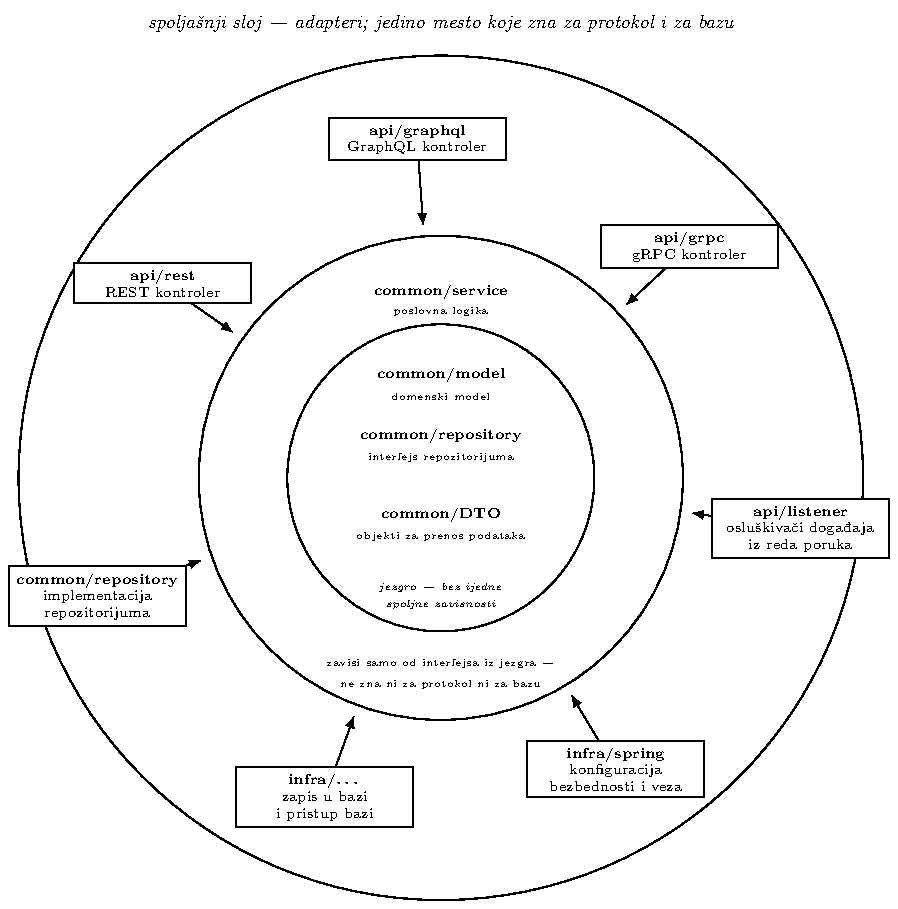
\includegraphics[width=0.95\textwidth]{slika-onion}
\documentclass[border=4pt]{standalone}
\usepackage[T1]{fontenc}
\usepackage[utf8]{inputenc}
\usepackage[english,serbian]{babel}
\usepackage{tikz}
\usetikzlibrary{arrows.meta,positioning}

\tikzset{
  kutija/.style={draw=black,line width=0.5pt,align=center,inner sep=3pt,
                 fill=white,font=\scriptsize,minimum width=3.0cm},
  str/.style={-{Latex[length=1.9mm,width=1.5mm]},line width=0.5pt,black},
}

\begin{document}
\begin{tikzpicture}

  % ---------- PRSTENOVI ----------
  \draw[line width=0.6pt] (0,0) circle (7.15);
  \draw[line width=0.6pt] (0,0) circle (4.1);
  \draw[line width=0.6pt] (0,0) circle (2.6);

  % ---------- JEZGRO ----------
  \node[align=center,font=\scriptsize\bfseries] at (0,1.75) {common/model};
  \node[align=center,font=\tiny] at (0,1.38) {domenski model};

  \node[align=center,font=\scriptsize\bfseries] at (0,0.72) {common/repository};
  \node[align=center,font=\tiny] at (0,0.35) {interfejs repozitorijuma};

  \node[align=center,font=\scriptsize\bfseries] at (0,-0.62) {common/DTO};
  \node[align=center,font=\tiny] at (0,-0.99) {objekti za prenos podataka};

  \node[align=center,font=\tiny\itshape] at (0,-1.85) {jezgro --- bez ijedne};
  \node[align=center,font=\tiny\itshape] at (0,-2.15) {spoljne zavisnosti};

  % ---------- SREDNJI PRSTEN ----------
  \node[align=center,font=\scriptsize\bfseries] at (0,3.15) {common/service};
  \node[align=center,font=\tiny] at (0,2.82) {poslovna logika};
  \node[align=center,font=\tiny] at (0,-3.15) {zavisi samo od interfejsa iz jezgra ---};
  \node[align=center,font=\tiny] at (0,-3.50) {ne zna ni za protokol ni za bazu};

  % ---------- SPOLJNI PRSTEN ----------
  \node[kutija] (krest)   at (145:5.75) {\textbf{api/rest}\\REST kontroler};
  \node[kutija] (kgql)    at (94:5.75)  {\textbf{api/graphql}\\GraphQL kontroler};
  \node[kutija] (kgrpc)   at (43:5.75)  {\textbf{api/grpc}\\gRPC kontroler};
  \node[kutija] (klisten) at (352:6.15) {\textbf{api/listener}\\osluškivači događaja\\iz reda poruka};
  \node[kutija] (kspring) at (301:5.75) {\textbf{infra/spring}\\konfiguracija\\bezbednosti i veza};
  \node[kutija] (kbaza)   at (250:5.75) {\textbf{infra/\dots}\\zapis u bazi\\i pristup bazi};
  \node[kutija] (kimpl)   at (199:6.15) {\textbf{common/repository}\\implementacija\\repozitorijuma};

  % ---------- STRELICE ----------
  % krecu od ivice kutije i staju tik iznad srednjeg prstena,
  % pa ne seku ni okvire ni tekst unutar prstena
  \draw[str] (krest)   -- (145:4.3);
  \draw[str] (kgql)    -- (94:4.3);
  \draw[str] (kgrpc)   -- (43:4.3);
  \draw[str] (klisten) -- (352:4.3);
  \draw[str] (kspring) -- (301:4.3);
  \draw[str] (kbaza)   -- (250:4.3);
  \draw[str] (kimpl)   -- (199:4.3);

  % ---------- NATPIS ----------
  \node[align=center,font=\small\itshape] at (0,7.7)
       {spoljašnji sloj --- adapteri; jedino mesto koje zna za protokol i za bazu};

\end{tikzpicture}
\end{document}
